\documentclass[10pt,a4paper]{article}
\usepackage[utf8]{inputenc}
\usepackage{amsmath}
\usepackage{amsfonts}
\usepackage{amssymb}
\usepackage{graphicx}
\usepackage{subcaption}

\begin{document}



\newpage
\tableofcontents
\newpage

\section{Introduction}
this is introduction
\section{Installation}
This section covers compiling LSBPT from source.

LSBPT is a Qt Widgets application developed with qt4, it has been tested under Linux ( fedora 23) and Mac OSX. It depends on several external libraries, listed below with version I used, other version libraries may also work.
\begin{itemize}
	\item opencv 2.4.12.2
	\item gdal 2.0.2
	\item OpenMP (gcc-4.9.2) \ Optimal. if not enabled, there may be some warnings " ignoring \#pragma omp ..."
\end{itemize}

Edit the "LSBPT.pro" in src folder to configure the library dependencies. 

\subsection{Linux and Mac OS X}
Once you solve the dependencies , follow the instructions to compile.
\begin{itemize}
	\item git clone 
	\item cd to the directory \ $\sim$/lsbpt
	\item \textit{ mkdir build } \ Create a build directory
	\item \textit{ cd build } \ Cd to build
	\item \textit{ qmake ../src } \ Use qmake to create makefile
	\item \textit{ make } Compile
	\item \textit{ chmox +x apps/LSBPT } \ Make the file executable
\end{itemize}
After compiling, you'll find the executable file "LSBPT" in ~/lsbpt/build/apps, simply type " \textit{path/to/LSBPT} " (i.e, \textit{app/LSBPT}  if you are in build directory) in bash to launch the application.

If you are using Qt creator, simply use "Open project" and select the "LSBPT.pro" under 
" \textit{$\sim$/lsbpt/src} ", then follow the instructions to configure  and compile the project.



\section{Run a segmentation}
Luanch the application simply by double click or with command line \\
\textit{path/to/the/application/LSBPT}, an interface is showed in figure \ref{fig:interface}. Click the first "..." button to select a image you want to segment and click second "..." to select a directory where you want to save the results, and then click  button "Go", a segmentation is running. When it finishes, a dialogue like figure \ref{fig:done} pops up reminding you the segmentation has been done.

\begin{figure}
\centering
	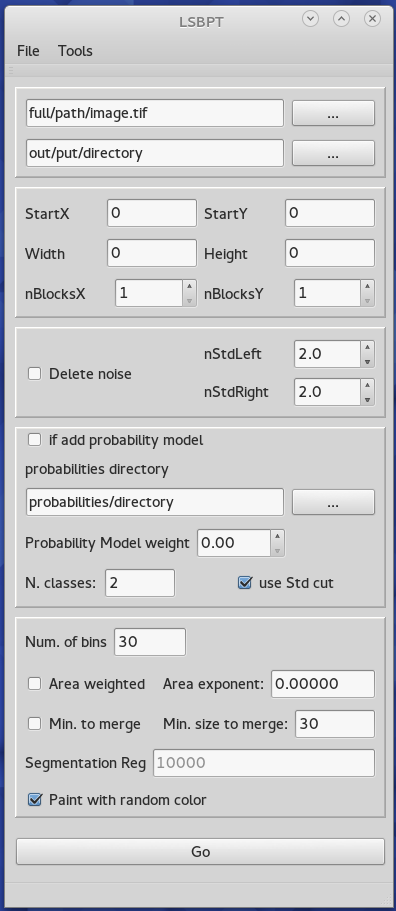
\includegraphics[scale=0.6]{figs/interface.png}
\caption{Software interface}
 \label{fig:interface}
\end{figure}

\begin{figure}
\centering
	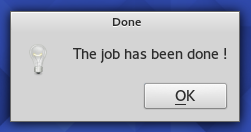
\includegraphics[scale=1]{figs/done.png}
\caption{Dialogue of finishing}
 \label{fig:done}
\end{figure}

\subsection{ Processing a part of the image}

It is possible to process any rectangular part of the image. The input "StartX" and "StartY" indicate the coordinates of left-up corner pixel of the rectangle part of horizontal and vertical direction respectively. Coordinates are set in up-down, left-right manner ( (0,0) at the left-up corner pixel of the image). "Width" and "Height" indicate the size of the rectangle you want to process. \textbf{We use 0 to indicate the rest part of the image start from "StartX" and "StartY"}. 

\subsection{ Processing with tiling strategy}

"nBlocksX" and "nBlocksY" indicates the number of tiles to split the image into in X and Y direction respectively. The image is split evenly, except that tiles in the last column and last row will may little bit larger if the size of the image can't be divided by the number of the tiles, please reference \textit{blockSizeCalculator\textunderscore evenSplite} function in "image" class for details.


\subsection{ Delete outliers }

If you want to delete some outliers, check the check box "Delete noise", "nStdLeft" and "nStdRight" indicates the number of standard deviation on each side. In this case, for each channel, pixel intensities which are larger than "mean + nStdLeft * sigma" will be set to "mean + nStdRight * sigma " and pixel intensities which are smaller than "mean - nStdLeft * sigma" will be set to "mean - nStdLeft * sigma", here "mean" is the mean value of the pixel intensities of the channel , "sigma" is the standard deviation.

\subsection{ Parameters for constructing BPTs and segmentation}

\begin{itemize}
	\item Num. of bins \ Indicates the number of bins of the histogram in histogram model
	\item Area weighted \ If use area when compute the dissimilarities between regions, check 				\textit{getOrder()} function in "compoundModel" class. This term is for balancing the tree.
	\item Area exponent \ The strength of using area to balance the tree
	\item Min. to merge (check box) \ If use minimum size to merge strategy
	\item Min. to merge \ If use minimum size to merge strategy, then regions which are smaller
	than this number will merge first. This strategy is also for balancing the tree, and it's also effective to eliminate some small segments
	\item Segmentation Reg \ Segmentation ( Classification ) regularization term. 
\end{itemize}



\subsection{ Multi-scale segmentation and classification }

LSBPT can extract multi-level segmentation or classification at the same time. The level is controlled by the regularization term ( \textbf{ Segmentation Reg} ). Several regularization term can be used at the same time, separated with ";" an example showed in \ref{fig:multi-scale}. An descending order is recommended though not mandatory. Results will be save with names
"segmentation+level.tif". "level" is set starting from 0. For example, if the regularization term is set to be "10000; 50000; 2000", then "segmentation0.tif" corresponding to 50000, and "segmentation1.tif corresponding to 10000, and "segmentation2.tif" corresponding to 2000.

\begin{figure}
\centering
	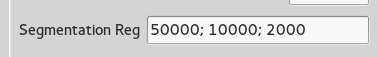
\includegraphics[scale=1]{figs/multi-scale.png}
\caption{ Input regularization term for multi-scale segmentation }
 \label{fig:multi-scale}
\end{figure}


\subsection{ Add probability model }

When probabilities are available,  we can add probability model. Double floats are used for probabilities, and they are written into binary file row-wise. Some example of the probability files are showed in "test/input/probabilities",  check loadProbabilities() function in "imageblock" class for more details.. 
For tiling strategy, each tiles has a probability file, and it is named as "i+indexX+j+indexY.dat" ( for example for a tile in the second column and third row, the name would be "i1j2.dat").

To add probability model, check the check box " if add probability model ", and select the directory where the probability files are saved. The other parameters are :

\begin{itemize}
	\item Probability Model weight \ This parameter indicates the importance of the probability model
	\item N. classes \ Number of classes 
\end{itemize}




























\end{document}